\item\problemnumber{NL6}{3}{30}{\ }{-}
Create the K-maps and then simplify for the following functions:
\begin{list}{\textbf{\alph{enumii}}}{\usecounter{enumii}}
    \item $F(x,y,z)=\overline{x}\,\overline{y}\,\overline{z}+\overline{x}yz+
    \overline{x}y\overline{z}$
    \item $F(x,y,z)=\overline{x}\,\overline{y}\,\overline{z}+
    \overline{x}y\overline{z}+x\overline{y}\,\overline{z}+xy\overline{z}$
    \item $F(x,y,z)=\overline{y}\,\overline{z}+\overline{y}z+xy\overline{z}$
\end{list}
\vskip12pt
\ifanswers
\textcolor{blue}{
\textbf{Answer:}\\
\begin{list}{\textbf{\alph{enumii}}}{\usecounter{enumii}}
    \item Here is a sample (problem 28a):\\[6pt]
        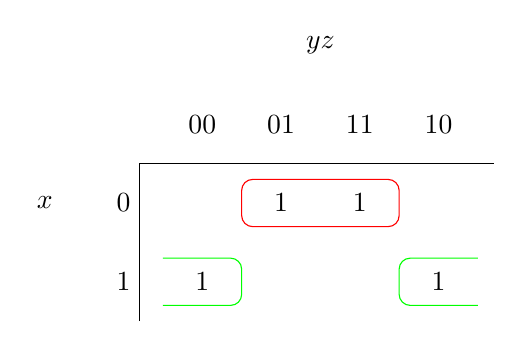
\begin{tikzpicture}
        \node at (3.5,3) {$yz$};
        \node at (2,2) {$00$};
        \node at (3,2) {$01$};
        \node at (4,2) {$11$};
        \node at (5,2) {$10$};
        \node at (0,1) {$x$};
        \node at (1,0) {$1$};
        \node at (1,1) {$0$};
        \node at (3,1) {$1$};
        \node at (4,1) {$1$};
        \node at (2,0) {$1$};
        \node at (5,0) {$1$};
        \draw (1.2,-0.5) -- (1.2,1.5) -- (5.7,1.5);
        \draw[color=green,rounded corners] (5.5,0.3) -- (4.5,0.3) -- (4.5,-0.3) -- (5.5,-0.3);
        \draw[color=green,rounded corners] (1.5,0.3) -- (2.5,0.3) -- (2.5,-0.3) -- (1.5,-0.3);
        \draw[color=red,rounded corners] (2.5,1.3) rectangle (4.5,0.7);
    \end{tikzpicture}
    \vskip12pt
    The resulting simplfied function is $F=\overline{x}z+x\overline{z}$\\[12pt]
    \item Part b answer goes here\\[12pt]
    \item Part c answer goes here\\[12pt]
\end{list}
}
\newpage
\fi
